\documentclass[12pt,a4paper]{cibb}
\usepackage{graphicx}
\usepackage{epstopdf}
\usepackage{caption}
\usepackage{ctable}
\usepackage{multirow}
\usepackage{hhline}
%\usepackage[utf8]{inputenc}
\usepackage{algorithm}
\usepackage{algorithmic}
\usepackage{setspace} 
%\usepackage{fullpage}
%\usepackage[top=1.5in, bottom=1.5in, left=1in, right=1in]{geometry}
\epstopdfsetup{outdir=./}
\usepackage{subfigure,graphicx}
\usepackage{pdflscape}
\usepackage{amsmath,amsfonts,latexsym,amssymb,euscript,xr}


\title{\large $\ $\\ \bf Improving genome assemblies using multi-platform sequence data}

\author{ P\i nar Kavak\,$^{1,2,}$\footnote{to whom correspondence should be addressed},  Bekir Erg\"{u}ner\,$^{1}$,  Duran \"{U}stek\,$^{3}$,  Bayram Y\"{u}ksel\,$^{4}$, \\
  Mahmut \c{S}amil Sa\u{g}\i ro\u{g}lu\,$^1$, 
  Tunga G\"{u}ng\"{o}r\,$^{2}$, and 
  Can Alkan\,$^{5,*}$}
\address{$\ $\\(1) Advanced Genomics and Bioinformatics Research Group (\.{I}GBAM)\\
B\.{I}LGEM, The Scientific and Technological Research Council of Turkey (T\"{U}B\.{I}TAK), 41470 Gebze, Kocaeli, Turkey, pinar.kavak@tubitak.gov.tr\\
%
\bigskip
(2) Department of Computer Engineering\\
Bo\u{g}azi\c{c}i University, 34342 Bebek, \.{I}stanbul, Turkey\\
%
\bigskip
(3) Department of Medical Genetics\\
\.{I}stanbul Medipol University, 34810 Beykoz, \.{I}stanbul, Turkey\\
%
\bigskip
(4) T\"UB\.{I}TAK - MAM - GMBE (The Scientific and Technological Research Council of Turkey, Genetic Engineering and Biotechnology Institute), 41470 Gebze, Kocaeli, Turkey\\
%
\bigskip
(5) Department of Computer Engineering\\
Bilkent University, 06800 Bilkent, Ankara, Turkey, calkan@cs.bilkent.edu.tr
}

\abstract{\textit{de novo} assembly, assembly improvement, next generation multi-platform sequencing.
\\[17pt]
{\bf Abstract.} \textit{De novo} assembly using short reads generated by next generation sequencing technologies is still an open problem. Although there are several assembly algorithms developed for data generated with different sequencing technologies, and some that can make use of hybrid data, the assemblies are still far from being perfect. There is still a need for computational approaches to improve draft assemblies.
Here we propose a new method to correct assembly mistakes when there are multiple types of data obtained using different sequencing technologies that have different strengths and biases.
We apply our method to Illumina, 454, and Ion Torrent data, and also compare our results with existing hybrid assemblers, Celera and Masurca.}

\begin{document}
\thispagestyle{myheadings}
\pagestyle{myheadings}
\markright{\tt Proceedings of CIBB 2015}%check year

\section{\bf Scientific Background}

Since the introduction of high throughput next generation sequencing (NGS) technologies, traditional Sanger sequencing is being abandoned especially for large-scale sequencing projects.
Although cost effective for data production, NGS also imposes increased cost for data processing and computational burden. 
In addition, the data quality is in fact lower, with greater error rates, and short read lengths for most platforms. 
One of the main algorithmic problems to analyze NGS data is the \textit{de novo} assembly: i.e. ``stitching'' billions of short DNA strings into a collection of larger sequences, ideally the size of chromosomes. 
However, ``perfect'' assemblies with no gaps and no errors are still lacking due to many factors, including the short read and fragment (paired-end) lengths, sequencing errors in basepair level, and the complex and repetitive nature of most genomes. 
Some of these problems in \textit{de novo} assembly can be ameliorated through using data generated by different sequencing platforms, where each technology has ``strengths'' that may be used to fix biases introduced by others.

Overlap-layout-consensus (OLC) graph based assemblers \cite{celera:2000, sga:2012} work well on the long read assembly. Assemblers that are based on de Bruijn graphs \cite{velvetZerbino:2008, spadesBankevich:2012, allpaths:2008} are designed primarily for short reads. 
Several assemblers 
use multiple read libraries \cite{cabogMiller:2008, masurcaZimin:2013, mira} for better assembly construction. Additionally, strategies to merge different assemblies using different data sources into a single coherent assembly are described in literature (e.g. \cite{wang:2012}). Our method differs from that of \cite{wang:2012}, in both pre- and post-processing steps.

In this work, we propose a method to improve draft assemblies (i.e. produced using a single data source, and/or single algorithm) by incorporating data generated by different NGS technologies, and applying novel correction methods. To achieve better improvements, we exploit the advantages of both short but low-error-rate reads and long but erroneous reads. 
We show that correcting the contigs built by assembling long reads through mapping short and high quality read contigs produce the best results, compared to the assemblies generated by algorithms that use hybrid data.

\section{\bf Materials and Methods}
\label{meth}

A part of human chromosome 13 was cloned into a bacterial artificial chromosome (BAC) in a previous study. 
We sequenced the BAC clone separately using Illumina, Roche/454, and Ion-Torrent platforms (see Table \ref{tab:dataprop}). A ``gold standard'' reference assembly was also obtained using template-based assembly with Mira~\cite{mira} using Roche/454 data, which is then corrected using the Illumina reads. Since Roche/454 and Ion Torrent platforms have similar sequencing biases (i.e. problematic homopolymers), we separated this study into two different groups: Illumina \& 454 and Illumina \& Ion-Torrent, which gives us the opportunity to compare Roche/454 and Ion-Torrent data.

\ctable[
      cap     = {},
      % 
      caption = {Properties of the data},
      % 
      label   = {tab:dataprop},
      doinside = \normalsize,
      width = 0.95\textwidth,
      %
      %
      pos = h!tb,
      star
]      {>{\raggedright\arraybackslash}X>{\raggedright\arraybackslash}X>{\raggedright\arraybackslash}
X>{\raggedright\arraybackslash}X>{\raggedright\arraybackslash}}
{
      \tnote[]{\textbf{Technology}: The name of the sequencing technology used to produce the reads.
      \textbf{Length range}: Minimum and maximum lengths of the generated reads.
      \textbf{Mean length}: The mean length among all reads.
      \textbf{Mean base qual}: The average phred score sequence quality of all reads. Calculated by summing up all phred scores of the bases in a read and dividing 
      it to sequence length over all reads.
      \textbf{Paired:} Represents whether the sequencing is performed as paired-end or single-end.}
}
{ \FL
Technology & Length range & Mean length & Mean base qual (phred s.) & Paired \\ \ML
Illumina & 101bp \footnotesize{(all reads have equal length)} & 101bp & 38 & paired \\
\addlinespace[1mm]
Roche/454 & 40bp-1027bp & 650bp & 28 & single-end \\
\addlinespace[1mm]
Ion-Torrent & 5bp-201bp & 127bp & 24 & single-end \\
\LL
}
\textbf{Pre-processing:} First, the reads that has low average quality value (phred score 17, i.e. $\geq$2\% error rate) were discarded. Then, the reads with high N-density (with $>$10\% of the read consisting of Ns) were removed. Third, groups of bases that seem to be non-uniform according to sequence base content were trimmed. Finally, each assembler's pre-processing operations were also inevitably applied.

\textbf{Assembly:} Several assembly tools were used: Velvet\cite{velvetZerbino:2008}, a de Bruijn graph based assembler to assemble the short reads; and two different overlap-layout-consensus (OLC) assemblers: Celera~\cite{celera:2000}, and SGA~\cite{sga:2012} to assemble the long read data sets (Roche/454 and Ion Torrent) separately. In addition, a de Bruijn graph based assembler, SPAdes\cite{spadesBankevich:2012} was also used on the long read data. 
Then all draft assemblies were mapped to the E. coli reference sequence using BLAST\cite{blast} to identify and discard E. coli contamination due to the cloning process. At the end, one short read, and three long read assemblies were obtained.

\textbf{Correction:} We used BLAST \cite{blast}  to map the contigs obtained with the short reads onto the contigs generated by assembling the long reads. Since BLAST may report multiple mapping locations due to repeats, only the ``best'' map locations were accepted. Reasoning from the fact that the short reads show less sequencing errors, the sequence reported by the short read based contigs were preferred over the long read contigs when there are disagreements between the pair. By doing this, the ``less fragmented'' long read assemblies were patched. Figure \ref{correction} shows a visual representation of the strategy on correcting the long read contigs. The strategy we applied is as follows: if there is a mapping between a short read contig and a long read contig, and if the mapping does not start at the beginning of the long read contig, add the unmapped prefix of the long read contig. Also, if the mapping does not start at the beginning of the short read contig (very rare situation), add the unmapped prefix of the short read contig with lowercase letters. The reason for using lowercase letters is to keep track of the information that there is a disagreement between the short read contig and long read contig on these sections, so the basepair quality will be lower than other sections of the assembly. One may argue that it might disturb the continuity of the resulting contig, however, we observe such mapping properties  very rarely.
% koptum burada. cok da gerekli degil gibi:
% Then, add the mapping part of the short read contig, while discarding the mapping part of the long read contig. If the mapping does not end at the end of the short read contig (rare), add the last part of the short read contig, again with lowercase letters. Finally, add the unmapping end of the long read contig and obtain the corrected contig. This process was repeated for each of the three long read assembly data sets. 

\textbf{Evaluation:} We mapped each of the final corrected assemblies to the ``gold standard'' reference assembly we constructed (described above), and calculated various statistics based on the comparisons, and estimated assembly qualities (Table~\ref{tab:resultsTable}). We also used two hybrid assemblers, Celera-CABOG~\cite{cabogMiller:2008} and Masurca \cite{masurcaZimin:2013}, with the same data to compare our correction methodology with those of hybrid assembly algorithms.


\begin{figure*}[htbp]
\centerline{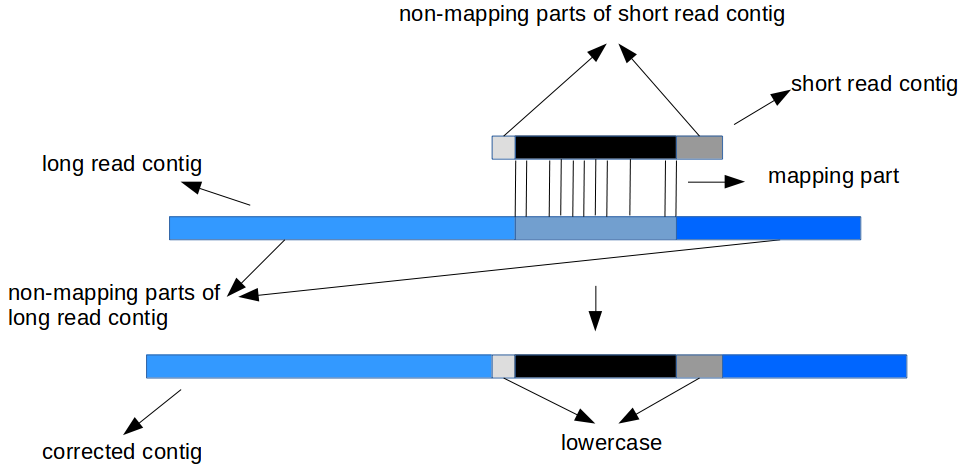
\includegraphics[width=12cm, height=5cm]{BACAlgorithm1.png}}
\caption{Correction method: Correct the long read contig according to the mapping information of the short read contig.}
\label{correction}
\end{figure*}

%\begin{algorithm}
%\caption{Assemble the query (short reads contig) and the subject (long reads contig) according to mapping information}
%\label{assembly}
%\begin{algorithmic} 
%\REQUIRE {mapping query and subject}
%\IF{the map does not start at the beginning of the subject}
%\STATE{add the unmapping beginning of the subject}
%\ENDIF
%\IF{the map does not start at the beginning of the query}
%\STATE {add the first part of the query to the result with lowercase letters}
%\ENDIF
%\STATE{add the mapping part of the query}
%\IF{the map does not end at the end of the query}
%\STATE{add the last part of the query to the result with lowercase letters}
%\ENDIF
%\IF{the map does not end at the end of the subject}
%\STATE{add the unmapping end of the subject}
%\ENDIF
%\end{algorithmic}
%\end{algorithm}

\section{\bf Results}
\label{res}
A summary of the results is presented in Table \ref{tab:resultsTable}. Briefly, the Velvet assembly using only the Illumina reads showed better coverage (99\%) and high average identity  (97.5\%) rates compared to Celera assembly using long reads. Correcting the Celera assembly with our method improves both coverage and average identity rates, which are then further improved by reiterative application of our method. 

The coverage of 454 assembly increases up to 99.7\% and the average identity rate increases up to 94.4\% on the first correction cycle. The repetitive correction cycles increase the coverage and average identity rates. The cycles are stopped if there is no improvement ($\geq 0.001$) or decrease on the average identity because of the increase on the coverage. One can see that correcting the long read assembly with the short read contigs works well with all kind of assemblers. However, corrected SGA assembly has the highest coverage rate among all.

Assembling short and long reads separately with de Bruijn and OLC graph based assemblers and correcting them give better results than assembling short and long reads together with a hybrid assembler such as Masurca or Celera. Masurca seems to have the best average identity rate on Illumina-Ion Torrent data, but the coverage for this run is just 1\%. Celera-CABOG performs very well on Illumina-454 data, but no better than corrected SGA or corrected Celera with Illumina and 454. Celera-CABOG does not have any contigs which successfully map onto the reference sequence, with Illumina-Ion-Torrent data, because all 487 resulting contigs were eliminated on the E.coli contamination filtering phase.

\ctable[star
	    center
      cap     = {},
      % 
      caption = {Results of assembly correction method on BAC data.},
      % 
      label   = {tab:resultsTable},
      doinside = \scriptsize,
      width = 1\textwidth,
      %maxwidth=19cm,
      %
      %
       pos = htb      
       ]
       {c>{\raggedright\arraybackslash}X>{\raggedright\arraybackslash}X>{\raggedright\arraybackslash}
         X>{\raggedright\arraybackslash}X>{\raggedright\arraybackslash}X>{\raggedright\arraybackslash}
         X>{\raggedright\arraybackslash}X>{\raggedright\arraybackslash}}
       {         
        \tnote[]{{\tiny Name: the name of the data group that constitute the assembly; \# of contigs: the number of contigs that belong to the resulting assembly; \# of Mapped Contigs: the number of contigs that successfully mapped onto the reference sequence; \# of Covered bases: the number of bases on the reference sequence that are covered by the assembly; Coverage: percentage of covered reference; Avg. identity: percentage of the correctly predicted reference bases; \# of Gaps: The number of gaps that cannot be covered on the reference genome; Size of Gaps: total number of bases on the gaps.}}
         \tnote[*]{{\tiny ``2'' represents the results of the second cycle of correction, ``3'' represents the third cycle.}}
       }
       {
         \FL
         Name & Length & \# of Contigs & \# of Mapped Contigs & \# of Covered bases & Coverage & Avg. Identity & \# of Gaps & Size of Gaps\ML
		 \textbf{\textit{Reference}} & \textit{176.843} & & & & & & & \ML
		 \addlinespace
		 \textbf{Velvet} & & & & & & & \NN
         Ill. Velvet & 197,040 & 455 & 437 & 175,172 & 0.99055 & 0.97523 & 39 & 1,671 \ML
         \textbf{Celera} & & & & & & & \NN       
         454 Celera & 908,008 & 735 & 735 & 172,563 & 0.97580 & 0.92599 & 18 & 4,280 \NN
         Ion Celera & 39,347 & 27 & 27 & 47,638 & 0.26938 & 0.96932 & 47 & 129,205 \ML
         \addlinespace
         \textbf{Corrected Celera} & & & & & & & \NN
         Ill-454 Celera & 4,945,785 & 895 & 270 & 176,368 & 0.99731 & 0.94370 & 5 & 475 \NN
         Ill-454 Celera^2\tmark[*] & 5,078,059 & 890 & 265 & 176,640 & 0.998852 & 0.944527 & 4 & 203 \NN
%         Ill-454 Celera^3 & 5,086,627 & 890 & 265 & 176,640 & 0.998852 & 0.944560 & 4 & 203 \NN
         Ill-Ion Celera & 93,909 & 30 & 28 & 81,819 & 0.46267 & 0.96327 & 36 & 95,024 \NN
         Ill-Ion Celera^2 & 145,262 & 30 & 28 & 91,962 & 0.52002 & 0.97412 & 33 & 84,881 \NN
         Ill-Ion Celera^3 & 216,167 & 30 & 28 & 99,645 & 0.56347 & 0.98066 & 34 & 77,198 \ML
         \textbf{SGA} & & & & & & & \NN
         454 SGA & 62,909,254 & 108,095 & 101,514 & 176,546 & 0.99832 & 0.97439 & 1 & 297 \NN
         Ion SGA & 842,997 & 6,417 & 6,122 & 153,092 & 0.86569 & 0.99124 & 197 & 23.751 \ML	
         \addlinespace
         \textbf{Corrected SGA} & & & & & & & \NN
         Ill-454 SGA & 295,009 & 335 & 335 & 176,757 & 0.99951 & 0.96823 & 5 & 86 \NN
         Ill-454 SGA^2 & 279,034 & 305 & 305 & 176,757 & 0.99951 & 0.96769 & 5 & 86 \NN
         Ill-Ion SGA & 197,509 & 291 & 291 & 175,052 & 0.98987 & 0.97501 & 45 & 1,791 \NN
         Ill-Ion SGA^2 & 203,064 & 291 & 291 & 175,676 & 0.99340 & 0.97413 & 34 & 1,167 \NN
%         Ill-Ion SGA^3 & 204,524 & 291 & 291 & 175,677 & 0.99341 & 0.97405 & 34 & 1,166 \ML
         \textbf{SPADES} & & & & & & & \NN
         454 SPADES & 12,307,761 & 49,824 & 49,691 & 176,843 & 1.0 & 0.98053 & 0 & 0 \NN
         Ion SPADES & 176,561 & 110 & 107 & 167,890 & 0.94937 & 0.92909 & 9 & 8,953 \ML	
         \addlinespace
         \textbf{Corrected SPADES} & & & & & & & \NN
         Ill-454 SPADES & 290,702 & 298 & 298 & 176,454 & 0.99780 & 0.96538 & 5 & 389 \NN
%         Ill-454 SPADES^2 & 290,917 & 297 & 297 & 176,454 & 0.99780 & 0.96530 & 5 & 389 \NN
%         Ill-454 SPADES^3 & 291.653 & 297 & 297 & 176.454 & 0.99780 & 0.96527 & 5 & 389 \NN
         Ill-Ion SPADES & 198,665 & 52 & 52 & 171,977 & 0.97248 & 0.94215 & 4 & 4,866 \NN
         Ill-Ion SPADES^2 & 200,307 & 52 & 52 & 172,101 & 0.97319 & 0.94230 & 2 & 4,742 \ML
         \textbf{Masurca} & & & & & & & \NN
         Ill-454 Masurca & 380 & 1 & 0 & 0 & 0 & 0 & 0 & 0 \NN
         Ill-Ion Masurca & 2,640 & 8 & 8 & 1,952 & 0.01104 & 0.98223 & 9 & 174,891 \ML
 		\textbf{Celera-CABOG} & & & & & & & \NN
         Ill-454 Celera & 1,101,716 & 891 & 891 & 174,330 & 0.98579 & 0.92452 & 12 & 2,513 \NN
         Ill-Ion Celera & 0 & 0 & 0 & 0 & 0.0 & 0.0 & 0 & 0.0 \ML
         \LL
       }
\vspace*{-0.3cm}

\section{\bf Conclusion}

Assembly correction by using advantages of different technologies improves the resulting assembly. Here we presented a new method to improve draft assemblies by correcting high contiguity assemblies using high quality short read contigs. 

Our results show that our method is useful and it gives better results than using all data for once with a hybrid assembler compared to the results of two hybrid assemblers. However, the need to develop new methods that exploit different data properties of different NGS technologies, such as short/long reads or high/low quality of reads, remains. In this manner, as future work, our correction algorithm can be improved by exploiting the paired end information of the short, high quality reads after the correction phase, to fill in the gaps between corrected contigs.

\section*{\bf Funding}
The project is supported by the Republic of Turkey Ministry of Development Infrastructure Grant (no: 2011K120020), B\.{I}LGEM \-- T\"{U}B\.{I}TAK (The Scientific and Technological Research Council of Turkey) grant (no: T439000), and a T\"{U}B\.{I}TAK grant to C.A.(112E135).\\

\newpage

\bibliographystyle{apalike}
{\fontsize{10}{10}\selectfont
\begin{thebibliography}{99}
\setlength{\parskip}{0pt}

\bibitem{celera:2000} E.W.Myers \textit{et~al} (2000) A Whole-Genome Assembly of Drosophila, \textit{Science}, {287(no:5461)}:2196-2204, doi:10.1126/science.287.5461.2196.
\bibitem{sga:2012} J.Simpson \textit{et~al} (2012) Efficient \textit{de novo} Assembly of Large Genomes Using Compressed Data Structures, \textit{Genome Research}, {22}:549-556, doi:10.1101/gr.126953.111.
\bibitem{velvetZerbino:2008} D.Zerbino, E.Birney (2000) Velvet: Algorithms for \textit{de novo} Short Read Assembly Using de Bruijn Graphs, \textit{Genome Research}, {18(5)}:821-829, doi: 10.1101/gr.074492.107.
\bibitem{spadesBankevich:2012} A.Bankevich {\it et~al} (2012) SPAdes: A New Genome Assembly Algorithm and Its Applications to Single-Cell Sequencing, \textit{Journal of Computational Biology}, {19(5)}:455-477, doi:10.1089/cmb.2012.0021.
\bibitem{allpaths:2008} J.Butler \textit{et~al} (2008) ALLPATHS: \textit{De novo} Assembly of Whole-Genome Shotgun Microreads, {\it Genome Research}, {18(5)}:810-820, doi:10.1101/gr.7337908.
\bibitem{cabogMiller:2008} J.R.Miller \textit{et~al} (2008) Aggressive Assembly of Pyrosequencing Reads with Mates, \textit{Bioinformatics}, {24(24)}:2818-2824, doi:10.1093/bioinformatics/btn548.
\bibitem{masurcaZimin:2013} A.Zimin \textit{et~al} (2013) The MaSuRCA Genome Assembler, \textit{Bioinformatics}, {29(21)}:2669-2677, doi:10.1093/bioinformatics/btt476.
\bibitem{mira} B.Chevreux {\it et~al} (1999) Genome Sequence Assembly Using Trace Signals and Additional Sequence Information, \textit{Computer Science and Biology:Proceedings of the German Conference on Bioinformatics (GCB)}, {99}:45-56.
\bibitem{wang:2012} Y.Wang {\it et~al} (2012) Optimizing Hybrid Assembly of Next-Generation Sequence Data from Enterococcus Faecium: a Microbe with Highly Divergent Genome, \textit{BMC Systems Biology}, {6(Suppl 3)}:S21, doi:10.1186/1752-0509-6-S3-S21. 
\bibitem{blast} S.Altschul {\it et~al} (1990) Basic Local Alignment Search Tool, \textit{Journal of Molecular Biology}, {215(3)}:403-410.

\end{thebibliography}
}
\end{document}



